
\section{Theory of Decision Trees}

In this section a (computer) scientific base for the informal introduction of decision trees shall be given. As mentioned in the introduction a basic knowledge in graph theory, machine learning and computer science in general is assumed.


\subsection{Definitions}

\begin{definition}
A \textbf{tree} is a directed, connected graph with one root node. Every other node has a single predecessor (\textbf{parent}) and no or more successors (\textbf{children}). Nodes without successors are called \textbf{leaves}. All nodes are connected by \textbf{edges}. The \textbf{depth} of a node is the number of edges on the path to the root. The \textbf{height} of the whole tree is the number of edges on the longest path from the root to any leaf. 
\end{definition}

\begin{remark}
This very rough definition focussed on trees shall not hide the fact that graph theory is complex and enormous mathematical field. For a deeper look e.g. \cite{cormen2001introduction} is recommended.
\end{remark}

\begin{definition}
A \textbf{decision tree} is a tree with following equivalents:
\begin{center}
\begin{tabular}{l|l} 
    \textbf{Tree} &  \textbf{Decision tree equivalent} \\ \hline
    Root & Initial decision node  \\ 
    Node & Internal decision node for testing on an attribute  \\ 
    Edge & Rule to follow \\ 
    Leaf & Terminal node represents the resulting classification 
\end{tabular}
\end{center}
\end{definition}

As mentioned in subsection \ref{taxonomy}, machine learning is a set of algorithms that extract models representing patterns from data and then evaluate those models. Let us define four relevant terms, which are important for understanding the following algorithms descriptions: instance, attribute, class, and dataset:

\begin{definition}
    The input of a machine learning algorithm consists of a set of \textbf{instances} (e.g. rows, examples or observations). Each instance is described by a fixed number of \textbf{attributes} (i.e. columns), which are assumed to be either nominal or numeric, and a label which is called \textbf{class} (in case of a classification task). The set of all instances is called \textbf{dataset}.
\end{definition}

Following this definition we get a table containing the dataset: Each decision becomes an attribute (all binary relations), all leaves are classes, while each row represents an instance of the dataset (see table \ref{tab:decisiontable}).

\begin{table}[!h] \centering
\begin{tabular}{|l| l l l |l|} \hline
    \textbf{Instance} & \multicolumn{3}{c|}{\textbf{Attribute}} & \multicolumn{1}{c|}{\textbf{Class}}\\ 
    & $A<B$ & $B<C$ & $A<C$ &  \\ \hline
    1 & yes & yes & yes & $A < B < C$ \\ 
    2 & yes & yes & no & $A < B < C$ \\
    3 & yes & no & yes & $A < C \leq B$ \\
    4 & yes & no & no & $C \leq A < B$ \\
    5 & no & yes & yes & $B \leq A < C$ \\ 
    6 & no & yes & no & $B < C \leq A$ \\
    7 & no & no & yes & $C \leq B \leq A$ \\
    8 & no & no & no & $C \leq B \leq A$ \\ \hline
\end{tabular}
\caption{Dataset table for the sorting example from subsection \ref{whatisadecisiontree}}
\label{tab:decisiontable}
\end{table}

Normally, the transformation is vice versa: the data is collected in table form (e.g. databases) and a decision tree has to be generated. 

The reason why there are now eight instead of six classes is simple: it does not matter for instances 1, 2 and 7, 8, if $A<B$ or not; the result is the same class. This effect of removing irrelevant branches of a tree is called pruning and is also part of this paper (see \ref{treepruning}). 


\newpage

\subsection{Decision Tree Learning}

In this subsection the question how to generate a decision tree from a given dataset in general shall be answered.

A founding idea of tree-based classification is based in the Concept Learning System \cite{quinlan1986induction}.
All algorithms introduced in the next section are based on a simple but very powerful algorithm called TDIDT which stands for \textit{Top-Down Induction of Decision Trees} \cite{quinlan1986induction}. This algorithm framework consists of two methods, growing and pruning a decision tree, which are introduced in the next two pseudocode listings and follows the idea of divide and conquer \cite[p. 33]{cormen2001introduction}. 

\begin{remark}
    $\sigma$ is the relational operator for selection. See e.g. \cite[p. 145]{rob2008database} for further operators and more detailed information. 
\end{remark}

 
\begin{algorithm}
\SetKwInOut{Input}{Input}
\SetKwInOut{Output}{Output}
\SetKwFunction{treePruning}{treePruning}
\SetKwFunction{treeGrowing}{treeGrowing}
\SetKwFunction{stoppingCriterion}{stoppingCriterion}
\SetKwFunction{splittingCriterion}{splittingCriterion}
\Input{Training set $X$, attribute set $A$, target feature $y$}
\Output{Decision tree}
\BlankLine
Create a new tree $T$ with a single root node.\\
\eIf{\stoppingCriterion{$X$}}{
    Mark $T$ as a leaf with the most common value in $X$ as a label.
}{
    $\forall a_i \in A$ find \textcolor{faured}{$a$} that obtain the best \splittingCriterion{$a_i, X, y$}.\\
    Label $n$ with $a$.\\
    \For{each outcome \textcolor{faublue}{$v_i$} of \textcolor{faured}{$a$}}{
        Set subtree \textcolor{faugreen}{$t_i$} = \treeGrowing{$\sigma_{a=v_i}X, A, y$}. \\
        Connect the root node of $n_t$ to the subtree \textcolor{faugreen}{$t_i$} with an edge that is labelled as \textcolor{faublue}{$v_i$}.
    }
}
\Return{\treePruning{$S, T, y$}}
\caption{Tree Growing \texttt{treeGrowing}}
\end{algorithm}

\begin{algorithm}
\SetKwInOut{Input}{Input}
\SetKwInOut{Output}{Output}
\SetKwFunction{pruned}{pruned}
\Input{Training set $X$, tree to be pruned $T$, target feature $y$}
\Output{Decision tree}
\BlankLine
\Repeat{$t = \emptyset$}{
      Select a node $n$ in $T$ such that pruning this node $n$ maximally improves some evaluation criterions. \\
    \If{$n \neq \emptyset$}{
        $T = $ \pruned{$T, n$}
    }
}
\Return{$T$}
\caption{Tree Pruning \texttt{treePruning}}
\end{algorithm}


A simplified decision tree \ref{fig:frameworktree} created by this algorithmic framework shall clarify how it works. The colors correspond to the variables in the pseudocode.

\begin{figure}[!h] \centering
\begin{tikzpicture}[
    level distance=2cm,
    level 1/.style={sibling distance=2.5cm},
    level 2/.style={sibling distance=4cm},
    leaf/.style={isosceles triangle,dashed,shape border rotate=90,isosceles triangle stretches=true, minimum height=20mm,minimum width=20mm,inner sep=0,yshift={-20mm}}]
\tikzstyle{every node}=[rectangle,draw]    
\node (Root) {\textcolor{faured}{$a$}}
child[child anchor=north] { 
    node[leaf] {\textcolor{faugreen}{$t_1$}}
    edge from parent node[left,draw=none] {\textcolor{faublue}{$v_1\;$}}
}
child[child anchor=north] { 
    node[leaf] {\textcolor{faugreen}{$t_2$}}
    edge from parent node[right,draw=none] {\textcolor{faublue}{$v_2$}}
}
child[child anchor=north] { 
    node[leaf, text height=1.5em] {$\dots $}
    edge from parent node[right,draw=none] {$\dots$}
}
child[child anchor=north] { 
    node[leaf] {\textcolor{faugreen}{$t_n$}}
    child[grow=right, xshift={10mm}] {
        node[draw=none]{Subtrees}
        edge from parent[draw=none]
        child[grow=up, yshift={7.5mm}] {
            node[draw=none]{Values of \textcolor{faured}{$a$}}  
            edge from parent[draw=none]
            child[grow=up, yshift={-7.5mm}] {
                node[draw=none]{Best attribute in $A$}  
                edge from parent[draw=none]
            } 
        }    
    }
    edge from parent node[right,draw=none] {\textcolor{faublue}{$v_n$}}
}
;
\end{tikzpicture}
\caption{The basic structure of a decision tree created by the algorithmic framework.}
\label{fig:frameworktree}
\end{figure}


This framework gives three positions to adjust the framework: the splitting and the stopping criterion, as well as the tree is going to be pruned. The following parts shall give a quick overview of these positions. 

\newpage

\subsubsection{Splitting Criterion}

All introduced criterions are based on impurity measure. This defines how well classes are separated. 

\begin{remark}
 For further information about impurity based criterions \cite[p. 53 ff.]{rokach2008data} is highly recommended.
\end{remark}

Of course, it is not possible to list all criterions and ideas for splitting in the scope of this short paper. The selected criterions are needed for the presented algorithms in section \ref{selectedalgorithms}. 

Comparison of splitting criterions is a frequently visited research topic (e.g. \cite{breiman1996technical}, \cite{buntine1992further}, \cite{mingers1989empirical}, \cite{drummond2000exploiting}, \cite{shih1999families}). Although, there is no extraordinary difference, each splitting criterion is superior in some cases and inferior in others; a general, scientifically sound statement which one is ``better'' is not possible. 

For the different node splitting criterions we introduce some notation used throughout this section.

We assume there are total number of $C$ classes denoted by $\Omega = {\omega_1, \omega_2, \dots, \omega_C}$. Let there be $N$ training examples represented by
\begin{equation}
    \left(x^{(1)}, y^{(1)} \right), \left(x^{(2)}, y^{(2)} \right), \dots, \left(x^{(N)}, y^{(N)} \right)
\end{equation}
where $x^{(i)}$ is a vector of $n$ attributes and $y^{i} \in \Omega$ is the class label corresponding to the input $x^{(i)}$. Of these $N$ examples, $N_{\omega_k}$ belong to the class $\omega_k$, while $\sum_k N_{\omega_k} = N$. The decision rule splits these examples into $P$ partitions, or $P$ child nodes, each of which has $N^(p)$ examples. The number of examples in a particular partition $p$ is denoted by $N^{(p)}_{\omega_k}$, while $\sum_k N^{(v)}_{\omega_k} = N^{(p)}$.


\paragraph{Entropy \& Information Gain}

The idea of the information gain is based on the information theory which was introduced by Claude Elwood Shannon in 1948 \cite{shannon2001mathematical}. For the computation we need two magnitudes: 


\begin{definition}
The \textbf{entropy} and the \textbf{information gain} are defined as

\begin{align}
    G(a_j) = \left( \sum_{k=1}^C -  \frac{N_{\omega_k}}{N} \log_2 \frac{N_{\omega_k}}{N}  \right) - \left( \sum_{p}^P \frac{N^{(p)}}{N} \cdot \sum_{k=1}^C -  \frac{N^{(p)}_{\omega_k}}{N^{(P)}} \log_2 \frac{N^{(p)}_{\omega_k}}{N^{(P)}} \right) \label{entropy}
\end{align}
while the first term is the entropy and the second term the weighted entropy of the child nodes. The difference thus reflects the decrease in entropy or the information gained from the use of attribute $a_j$.

%\begin{equation}
%    G_{\text{Entropy}}(a_i, S, y) = H(y, S) - \sum_{j \in a_i} \frac{\left|S_j\right|}{|S|} \cdot H(y, S_j)
%\end{equation}
%where
%\[
%    H(y, S) = - \sum_{k = 1}^{|y|} P(y_k) \log_2 P(y_k), \qquad S_j = \sigma_{a_j = j}S, \qquad P(y_k) = \frac{\left|\sigma_{y_k = y}S\right|}{|S|}
%\]

%and $j$ are all manifestations of $a_i$ and $y_k$ all classes of the feature vector $y$. 
\end{definition}

%In other words: $P(y_i)$ is the probability of occurrence of the class $y_i$ in all classes $y$ of the given training set, $S_j$ is a subset of $S$, where the attribute can only attain the value of $j$, and $\sum_{j \in a_i}$ represents a iteration through the set $a_i$ -- similar to a \texttt{foreach}-loop.

\begin{remark}
    There is a detailed example in the presentation slides which should clarify the application of the formula.
\end{remark}


One of the problems that arises is that the information gain criterion as defined in equation \ref{entropy} favors large number of partition $P$. So the an improvement was suggested by \cite{quinlan1993c4}, which is now used in the C4.5: instead of the information gain $G(a_j) / g$ is used, where

\begin{equation}
    g = \sum_{p=1}^P \frac{N^{(p)}}{N} \log_2 \frac{N^{(p)}}{N} \label{gainratio}
\end{equation}




\paragraph{Gini Index \& Gini Gain}

\begin{definition}
    The \textbf{Gini index} measures the divergences between the probability distributions of the target attributes values and is defined as
\begin{align}
    D(a_j) = \frac{1}{N}\left( \sum_{k=1}^{C}\sum_{p=1}^{P} \frac{\left( N_{\omega_k}^{(p)} \right)^2  }{N^{(p)}} - \sum_{k=1}^C \frac{\left( N_{\omega_k}\right)^2  }{N} \right)
\end{align}

%    \begin{align}
%        g(y, S) = 1- \sum_{k=1}^{|y|} \left( \frac{|\sigma_{y_k = y}S|}{|S|} \right) ^2
%    \end{align}
%    Analogous to the information gain, the \textbf{Gini gain} $G_{\text{Gini}}(a_i, S, y)$ is for selecting the best attribute $a_i$ is defined as
%    \begin{align}
%        G_{\text{Gini}}(a_i, S, y) = g(y, S) - \sum_{j \in a_i} \frac{|S_j|}{|S|} \cdot g(y, S_j) \;.
%    \end{align}
\end{definition}

The goal is to find a node which is the most ``pure'' one, i.e. has instances of a single class. Similar to the decrease in entropy and gain information used in the information gain based criterion, the impurity as given in \ref{} is used. The chosen attribute is one that has the largest decrease in impurity.


\paragraph{Twoing Criterion}

\begin{definition}

The binary twoing criterion maximizes the function

\begin{align}
    \frac{P(t_L) \cdot P(t_R)}{4} \cdot \left( \sum_{c \in a_i} \left| P(c|t_L) - P(c|t_R) \right| \right) ^2
\end{align}

for a node $t$, where $P(t_L)$ and $P(t_R)$ are the probability of going left or right, respectively, and $P(c|t_L)$ and $P(c|t_R)$ are the proportions of data points in $t_L$ and $t_R$ which belong to class $c$.

\end{definition} 

Figure \ref{fig:twoingcriterion} visualizes the used variables:

\begin{figure}[!h] \centering
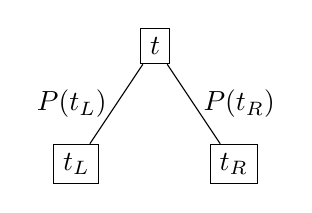
\begin{tikzpicture}[level distance=1.5cm,
level 1/.style={sibling distance=2cm},
level 2/.style={sibling distance=4cm}]
\tikzstyle{every node}=[rectangle,draw]    
\node (Root) {$t$}
child { 
    node {$t_L$}
    edge from parent node[left,draw=none] {$P(t_L)$}
}
child { 
    node {$t_R$}
    edge from parent node[right,draw=none] {$P(t_R)$}
};
%\node[draw=none] at (0,0.75) {$x_j \leq x^S_j$};
\end{tikzpicture}
\caption{Twoing criterion is a measure of the difference in probability that a category appears in the left descendant rather than the right descendant node. }
\label{fig:twoingcriterion}
\end{figure}

When the target attribute is binary the Gini and twoing criterion are equivalent \cite{shih1999families}. The towing rule is more appropriate for data, which has a large number of different classes. For multi-class problems the twoing criterion prefers attributes with evenly divided splits \cite[p. 57]{rokach2008data}.


\paragraph{Chi-Squared Statistic Criterion}

The chi-squared statistic ($\chi^2$) criterion is based on comparing the obtained values of the frequency of a class because of the split to the \textit{a priori} frequency of the class. 

\begin{definition}
The formula for computing the $\chi^2$ value is 
\begin{equation}
    \chi^2 = \sum_{k=1}^{C}\sum_{p=1}^{P} \frac{\left(\left| N_{\omega_k}^{(p)} \right| - \left| \tilde N_{\omega_k}^{(p)} \right| \right) ^2 }{ \left| \tilde N_{\omega_k}^{(p)} \right| }
\end{equation}
where $\tilde N_k^{(p)} = \cfrac{N^{(p)}}{N} \cdot N_{\omega_k}$ is the a priori frequency of the samples $N$ in $k$.
\end{definition}

A larger value of $\chi^2$ indicates that the split is more homogeneous, i.e. has a greater frequency of instances from a certain class. The attribute is chosen by the largest value of $\chi^2$.








\subsubsection{Stopping Criterion}

The growing phase continues until a stopping criterion is triggered. The following conditions are common stopping rules \cite[p. 63]{rokach2008data}:
\begin{itemize}
    \item All instances in the training set belong to a single value of $y$.
    \item The maximum tree depth has been reached.
    \item The number of cases in the terminal node is less than the minimum
number of cases for parent nodes.
    \item If the node were split, the number of cases in one or more child nodes
would be less than the minimum number of cases for child nodes.
    \item The best splitting criterion is not greater than a certain threshold.
\end{itemize}


\begin{remark}
    The last stopping criterion is used in the implementation for pruning after the growing phase.\label{stoppingcriterionimpl}
\end{remark}



\subsubsection{Tree Pruning}\label{treepruning}

Using a tight stopping criterion tends to create small and underfitted decision trees. On the other hand, using  loose stopping criterion tends to generate large decision trees that are overfitted to the training set. 

To avoid both extremes, the idea of pruning was developed: A loose stopping criterion is used and after the growing phase, the overfitted tree is cut back into a smaller tree by removing sub-branches that are not contributing to the generalization accuracy. 

Many approaches were developed and even the in the following presented ones have different versions with improvements. However, the focus is on the basic ideas. 


\paragraph{Reduced Error Pruning}

Reduced error pruning is a basic pruning approach introduced by Ross Quinlan in 1987 \cite{quinlan1987simplifying}. 

\begin{algorithm}[!h]
\SetKwInOut{Input}{Input}
\SetKwInOut{Output}{Output}
\SetKwFunction{treePruning}{treePruning}
\SetKwFunction{treeGrowing}{treeGrowing}
\SetKwFunction{stoppingCriterion}{stoppingCriterion}
\SetKwFunction{splittingCriterion}{splittingCriterion}
\Input{Training set $X$, attribute set $A$, target feature $y$}
\Output{Pruned decision tree}
\BlankLine
Subdivide $X$ into a training set $X_T$ and validation set $X_V$.\\
Build a tree $T = $ \treeGrowing{$X_T, A, y$}.\\
Pass all of the training examples $X_V$ through the tree $T$ and estimate the error rate of each node $n$ using $X_V$.\\
Convert a node to a leaf if it would have lower estimated error then the sum of the errors of its children.\\
\Return{T}
\caption{Reduced Error Pruning}
\end{algorithm}

However the splitting into two sets is not welcome, because it reduces the size of training set. 


\paragraph{Cost-Complexity Pruning}

Proposed by Leo Breiman in 1984, the pruning method is also known as weakest link pruning or error-complexity pruning. Contrary to the reduced error pruning this pruning approach is not straight forward \cite[p. 64]{rokach2008data}. 

The idea is to consider the size and the estimated error rate of the tree. The total cost $C_\alpha (T)$ of tree $T$ is defined as

\begin{equation}
    C_\alpha (T) = R(T) + \alpha | \tilde T |, \qquad \alpha \geq 0 
\end{equation}

where $R(T)$ is the weighted summed error of the leafs of tree $T$ and $\alpha$ is penalty for the complexity of the tree $\tilde T$ (so called complexity parameter), while $\tilde T$ stands for all leaves in the tree $T$.

For a fixed value of $\alpha$ there is a unique smallest minimizing subtree $T(\alpha)$ of the complete tree $T_{\max}$, that fulfills the following two conditions \cite{mingers1989empirical}:

\begin{align}
    \kreis{1} \qquad & C_{\alpha}\left(T(\alpha)\right) = \min_{T \subseteq T_{\max}} C_\alpha(T) \\
    \kreis{2} \qquad & \text{ If } C_\alpha(T) = C_{\alpha}\left(T(\alpha)\right) \text{ then } T(\alpha) \subseteq T
\end{align}

The first condition says that there is no subtree of $T_{\max}$ with lower costs than $T(\alpha)$ at that $\alpha$. The second condition says that if more than one tree achieves the same minimum, the cost-complexity pruning selects the smallest tree. Since $T_{\max}$ is finite, there is a finite number of different subtrees $T(\alpha)$ of $T_{\max}$. A decreasing sequence of $\alpha$ for subtrees of $T_{\max}$ would look like 
\[
    T_1 \supseteq T_2 \supseteq T_3 \supseteq \dots \supseteq \{n\}
\]
with $n$ as the root node of $T$ and $T_n$ is the smallest subtree for $\alpha \in [\alpha_n, \alpha_{n+1})$.

\paragraph{Error-Based Pruning}

The goal is to improve the estimate of error on unseen data using only training set data. Hence if a node does not increase estimated error, we prune it.

The error estimate for a subtree is the weighted (based on how many instances of each there are) sum of the error estimates for all its leaves, defined by

\begin{equation}
    \varepsilon (T, S) = \varepsilon(T, S) + Z_\alpha \cdot \sqrt{ \frac{\varepsilon(T,S) \cdot \left( 1- \varepsilon(T,S) \right)}{|S|} }
\end{equation}


where $\varepsilon(T, S)$ denotes the misclassification rate of the tree $T$ on the training set $S$; $Z$ is the inverse of the standard normal cumulative distribution; and $\alpha$ is the desired significance level.


\begin{remark}
    Cost-complexity pruning and reduced error pruning tends to over-pruning, while error-based pruning tend to under-pruning \cite[p.68]{rokach2008data}.
\end{remark}



\newpage


\subsection{Selected Algorithms}\label{selectedalgorithms}

Before we immerse in the underlying theory, a small historical background of all shall be given. 

\begin{figure}[!h]
\begin{tikzpicture}[snake=zigzag, line before snake = 5mm, line after snake = 5mm]
%draw horizontal line   
\draw (-0.5,0) -- (15.5,0);

%draw vertical lines
\foreach \x in {0,8,10,11,15}
   \draw (\x cm,3pt) -- (\x cm,-3pt);

%draw nodes
\draw (0,0) node[below=3pt] {AID} node[above=3pt] {$1963$};
\draw (8,0) node[below=3pt] {CHAID} node[above=3pt] {$1980$};
\draw (10,0) node[below=3pt] {CART} node[above=3pt] {$1984$};
\draw (11,0) node[below=3pt] {ID3} node[above=3pt] {$1986$};
\draw (15,0) node[below=3pt] {ID4.5} node[above=3pt] {$1993$};
\end{tikzpicture}
\caption{Timeline of four basic algorithm families: \textsf{CHAID}, CART, ID3 and ID4.5}
\label{}
\end{figure}


\begin{remark}
    As in the considered parts of decision tree theory, this is not a complete summarization of all decision tree algorithms. Instead, basic and popular algorithms were selected and will be introduced in the following. 
\end{remark}




\subsubsection{Chi-squared Automatic Interaction Detector (CHAID)} 

In 1964, the statisticians John A. Sonquist and James N. Morgan introduced a first version of tree learning algorithm called Automatic Interaction Detection (AID) \cite{morgan1963problems}. 

Gordon V. Kass proposed a modification to AID in his paper from 1979 \cite{kass1980exploratory} called \textit{Chi-squared Automatic Interaction Detector} (CHAID). 

The basic improvement was splitting criterion: instead of the variance the $\chi^2$-test is used. Therefore, the partitions need not be a bisection.

CHAID handles missing values by treating them as a separate valid category and does not perform any pruning. A short introduction to handling missing attribute values will be given in subsection \ref{missingattributes}.


\subsubsection{Iterative Dichotomiser 3 (ID3)} 

The ID3 algorithm was developed by Ross Quinlan in 1986. It uses the information gain as splitting criterion and it does not apply any pruning procedure nor does it handle numeric attributes or missing values.


\subsubsection{Classification And Regression Tree (CART)} 

Leo Breiman published his idea of CART in 1984 \cite[p. 18]{rokach2008data}. As the name suggests CART supports also regression trees. This book provides a strong statistic foundation and revived the idea of CLS \cite[p. 435]{duda2012pattern}.

Two splitting criterions can be chosen: the twoing or Gini criterion \cite[p. 1]{shih1999families}. The obtained tree is pruned by cost-complexity pruning.  


\subsubsection{C4.5}

C4.5 is the updated version of ID3 by the same author \cite{Kohavi99decisiontree}. It uses also the information gain, but extends this by the option of handling missing value and continuous values. This new splitting criterion is called gain ratio (see formula \ref{gainratio}).

After the growing phase an error-based pruning is performed.



\begin{remark}
    There is a commercial successor of C4.5, called C5.0 \cite{Kohavi99decisiontree}, but it has not influenced the decision tree learning in the way Quinlan's two other algorithms did: no scientific papers about the C5.0 itself are findable. 
\end{remark}






\subsection{Discussion}

In this part, the usage of decision trees shall be discussed. The pro and con statements are very general and thus not very precise. There are several approaches to avoid or at least minimize the disadvantages and maximize the benefits and advantages, as mentioned in the previous parts.


\subsubsection{Advantages}

Also a lot of advantages can be recognized \cite[p. 73ff.]{rokach2008data}. Decision trees
\begin{itemize}
    \item are self-explanatory and can be converted into a set of rules, which is easy and fast to interpret, understand, and implement: A path from the root to a leaf is the explanation for the resulting classification which is given by the leaf (terminal node). 
    \item can handle both nominal and numeric input values.
    \item are capable of handling data sets with missing values.
    \item are a nonparametric method, which means that they have no assumptions about the space distribution and the classifier structure. 
\end{itemize}


\subsubsection{Disadvantages}
On the other hand, decision trees have disadvantages such as 
\begin{itemize}
    \item an over-sensitivity to the training set, to irrelevant attributes, and to noise.
    \item a requirement that the target attribute consists only of discrete values (in case e.g. ID3 or C4.5).
    \item a tending to perform well if a few highly relevant attributes exist, because decision trees use the divide and conquer method; but less so if many complex interactions are present. 
\end{itemize}






\subsection{Outlook}

This subsection is about what was not part of the considerations of this seminar paper, but, in the humble opinion of the author, is important or interesting for working with decision trees.

\subsubsection{Complexity \& Performance}

Like for all computer algorithms the time and space complexity is relevant. \cite{buhrman2002complexity} gives a broad overview of the complexity of decision trees in general. 

In the following some assumptions contain the wide field of complexity. We suppose that we have $n$ training instances, $m$ attributes, $O(n)$ nodes (up to one leaf per example), and the tree depth of $O(\log n)$. So the complexities are given by table \ref{tab:complexity}. 

\begin{table}[!h] \centering
\begin{tabular}{|p{6cm} | l|} \hline
Building a tree & $O(m \cdot n \log n )$ \\
Subtree replacement & $O(n)$ \\
Subtree raising & $O\left(n \cdot (n \log n)^2 \right)$ \\ 
\vspace*{-2em} \begin{itemize}\item \small{Every instance may have to be redistributed at every node
between its leaf and the root} \vspace*{-1em} \end{itemize} & $ \qquad O\left(n \log n \right)$ \\
\vspace*{-2em} \begin{itemize}\item \small{Cost for redistribution (on average)} \vspace*{-1em} \end{itemize} & $ \qquad O\left( \log n \right)$ \\ \hline \hline
Total Cost & $O(m \cdot n \log n ) + O\left(n \cdot (n \log n)^2 \right)$ \\ \hline
\end{tabular}
\caption{Complexity overview of a assumed decision tree}
\label{tab:complexity}
\end{table}

But \cite{su2006fast} showed that it is possible with a novel algorithm to achieve a time complexity of $O(m \cdot n)$.  


Due to the fact that there are many improvements for each algorithm, a general statement is not feasible. But several research approaches compare the performances of decision tree algorithms with each other (e.g. \cite{lavanya2011performance}, \cite{banfield2007comparison}, \cite{safavian1991survey}) and decision trees with other classification approaches (e.g. \cite{huang2003comparing}, \cite{curram1994neural}). 



\subsubsection{Missing Attributes}\label{missingattributes}

It is common, that classification problems have missing attributes during training, during classification, or both. Consider first training a tree classifier despite the fact that some training patterns are missing attributes. 

There are several approaches to handle missing values. Numerical values can be initialized by a meaningful value (minimum, maximum, average, $-1$, etc.). For nonnumerical attributes it might be useful to choose the commonest attribute value. 

For a more detailled description of the approaches to handle missing values, e.g. \cite{zhang2005missing} and \cite[p. 59 ff.]{rokach2008data} are recommended.


\subsubsection{Random Forests}

A Random forest is a classifier consisting of $n$ decision trees \cite{tong2003decision}. This method combines the \textit{Bagging} (\underline{B}ootstrap \underline{agg}regat\underline{ing}, \cite[p. 105ff.]{rokach2008data}) method and the random selection of features \cite[p. 87 ff.]{rokach2008data}. 

Figure \ref{fig:randomforest} gives a short graphical overview of the data flow and the functional principle of random forests.
 

\begin{figure}[!h] \centering
\begin{tikzpicture}[level distance=2cm,
level 1/.style={sibling distance=3.5cm},
level 2/.style={sibling distance=1cm,level distance=1.5cm},
edge from parent fork down, edge from parent/.style={draw,-latex}]
\tikzstyle{every node}=[rectangle,draw]
\node (Root) [] (A) {Original Data}
    child {
        node (pt1) {Prediction Tree 1}
        edge from parent node[above,draw=none] {Bootstrap 1}
    }
    child {
        node (pt2) {Prediction Tree 2}
        edge from parent node[above,draw=none] {Bootstrap 2}
    }
    child {
        node (pt3) [draw=none]{\dots}
        edge from parent node[above,draw=none] {\dots}
    }
    child {
        node (pt4) {Prediction Tree $n$}
        edge from parent node[above,draw=none] {Bootstrap $n$}
    }
;
\node[draw=none] (t) at (0,-3) {};
\node (df) at (0,-4) {Decision Forest};
\draw (pt1) |- (t.center);
\draw (pt2) |- (t.center);
\draw (pt3) |- (t.center);
\draw (pt4) |- (t.center);
\draw[draw, -latex] (t.center) -- (df);
\end{tikzpicture}
\caption{The random forest schematic}
\label{fig:randomforest}
\end{figure}


